We here only have an idea for an algorithm for solving this problem, it is not yet tested.

The algorithm is based an algorithm for solving the same problem in \cite{multiSearchSecure}, and the basic idea is to first place guards to break the problem down into smaller problems until a single guard can completely secure the smaller problem.
Once an area has been secured, it should never be allowed to be directly connected to unsecured areas again, but as long as this is satisfied, all guards may move around.
After securing an area, again try to break down the remaining problem into smaller problems and recurse.

\ \\
Each area has two different boolean properties:
\begin{definition}[Watched]
if at least one guard can see the whole area.
\end{definition}
\begin{definition}[Secured]
if all of it's neighbors are either secured or watched.
\end{definition}

Each guard only has one property:
\begin{definition}[Occupied]
if it is the only guard watching an area that is not secured itself, but connected to both secured and unsecured areas.
\end{definition}

\begin{algorithm}
This is an algorithm for finding the points for guards to visit in order to secure a given 2D vector environment divided into free-space and obstacles. Intruders are allowed to move arbitrarily fast.

The algorithm is greedy, but corresponding versions of searching for and evaluating different solutions could also be made.
\begin{enumerate}
	\item Tesselate the environment into convex polygons and generate a walkability-graph of the connected polygons. (see Figure \ref{searchDestroy})
	\item Somehow find a point $p$ which divides the graph into smaller graphs. (see Figure \ref{searchDestroy2})
			Preferably, at least one of the smaller graphs should be of a size smaller than the number of currently available unoccupied guards.
	\item Move an unoccupied guard to $p$, if all guards are occupied, add a new guard at $p$.
	\item If all the areas are either secured or watched, we are done, otherwise, goto 2.
\end{enumerate}
\qed
\label{algSearchDestroyIdea}
\end{algorithm}

The possible points to visit and how placing a guard at that point transforms the walkability-graph could possibly be pre-generated.

%\begin{figure}[h!t]
%	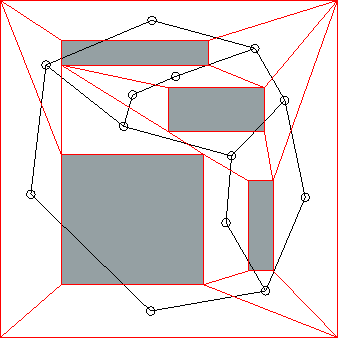
\includegraphics[width=\linewidth]{fig/2graph.png}
%	\caption{The tesselation (red) and walkability-graph (black) of an environment}
%	\label{searchDestroy}
%\end{figure}

%\begin{figure}[h!t]
%	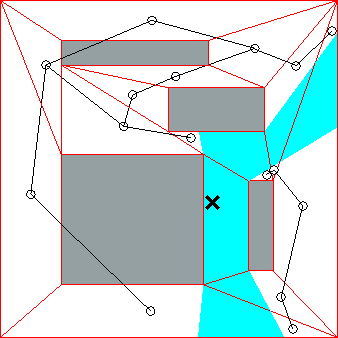
\includegraphics[width=\linewidth]{fig/2graph2.png}
%	\caption{The new walkability-graph after placing a guard at the cross}
%	\label{searchDestroy2}
%\end{figure}
